% Options for packages loaded elsewhere
\PassOptionsToPackage{unicode}{hyperref}
\PassOptionsToPackage{hyphens}{url}
%
\documentclass[
]{article}
\usepackage{amsmath,amssymb}
\usepackage{iftex}
\ifPDFTeX
  \usepackage[T1]{fontenc}
  \usepackage[utf8]{inputenc}
  \usepackage{textcomp} % provide euro and other symbols
\else % if luatex or xetex
  \usepackage{unicode-math} % this also loads fontspec
  \defaultfontfeatures{Scale=MatchLowercase}
  \defaultfontfeatures[\rmfamily]{Ligatures=TeX,Scale=1}
\fi
\usepackage{lmodern}
\ifPDFTeX\else
  % xetex/luatex font selection
\fi
% Use upquote if available, for straight quotes in verbatim environments
\IfFileExists{upquote.sty}{\usepackage{upquote}}{}
\IfFileExists{microtype.sty}{% use microtype if available
  \usepackage[]{microtype}
  \UseMicrotypeSet[protrusion]{basicmath} % disable protrusion for tt fonts
}{}
\makeatletter
\@ifundefined{KOMAClassName}{% if non-KOMA class
  \IfFileExists{parskip.sty}{%
    \usepackage{parskip}
  }{% else
    \setlength{\parindent}{0pt}
    \setlength{\parskip}{6pt plus 2pt minus 1pt}}
}{% if KOMA class
  \KOMAoptions{parskip=half}}
\makeatother
\usepackage{xcolor}
\usepackage[margin=1in]{geometry}
\usepackage{color}
\usepackage{fancyvrb}
\newcommand{\VerbBar}{|}
\newcommand{\VERB}{\Verb[commandchars=\\\{\}]}
\DefineVerbatimEnvironment{Highlighting}{Verbatim}{commandchars=\\\{\}}
% Add ',fontsize=\small' for more characters per line
\usepackage{framed}
\definecolor{shadecolor}{RGB}{248,248,248}
\newenvironment{Shaded}{\begin{snugshade}}{\end{snugshade}}
\newcommand{\AlertTok}[1]{\textcolor[rgb]{0.94,0.16,0.16}{#1}}
\newcommand{\AnnotationTok}[1]{\textcolor[rgb]{0.56,0.35,0.01}{\textbf{\textit{#1}}}}
\newcommand{\AttributeTok}[1]{\textcolor[rgb]{0.13,0.29,0.53}{#1}}
\newcommand{\BaseNTok}[1]{\textcolor[rgb]{0.00,0.00,0.81}{#1}}
\newcommand{\BuiltInTok}[1]{#1}
\newcommand{\CharTok}[1]{\textcolor[rgb]{0.31,0.60,0.02}{#1}}
\newcommand{\CommentTok}[1]{\textcolor[rgb]{0.56,0.35,0.01}{\textit{#1}}}
\newcommand{\CommentVarTok}[1]{\textcolor[rgb]{0.56,0.35,0.01}{\textbf{\textit{#1}}}}
\newcommand{\ConstantTok}[1]{\textcolor[rgb]{0.56,0.35,0.01}{#1}}
\newcommand{\ControlFlowTok}[1]{\textcolor[rgb]{0.13,0.29,0.53}{\textbf{#1}}}
\newcommand{\DataTypeTok}[1]{\textcolor[rgb]{0.13,0.29,0.53}{#1}}
\newcommand{\DecValTok}[1]{\textcolor[rgb]{0.00,0.00,0.81}{#1}}
\newcommand{\DocumentationTok}[1]{\textcolor[rgb]{0.56,0.35,0.01}{\textbf{\textit{#1}}}}
\newcommand{\ErrorTok}[1]{\textcolor[rgb]{0.64,0.00,0.00}{\textbf{#1}}}
\newcommand{\ExtensionTok}[1]{#1}
\newcommand{\FloatTok}[1]{\textcolor[rgb]{0.00,0.00,0.81}{#1}}
\newcommand{\FunctionTok}[1]{\textcolor[rgb]{0.13,0.29,0.53}{\textbf{#1}}}
\newcommand{\ImportTok}[1]{#1}
\newcommand{\InformationTok}[1]{\textcolor[rgb]{0.56,0.35,0.01}{\textbf{\textit{#1}}}}
\newcommand{\KeywordTok}[1]{\textcolor[rgb]{0.13,0.29,0.53}{\textbf{#1}}}
\newcommand{\NormalTok}[1]{#1}
\newcommand{\OperatorTok}[1]{\textcolor[rgb]{0.81,0.36,0.00}{\textbf{#1}}}
\newcommand{\OtherTok}[1]{\textcolor[rgb]{0.56,0.35,0.01}{#1}}
\newcommand{\PreprocessorTok}[1]{\textcolor[rgb]{0.56,0.35,0.01}{\textit{#1}}}
\newcommand{\RegionMarkerTok}[1]{#1}
\newcommand{\SpecialCharTok}[1]{\textcolor[rgb]{0.81,0.36,0.00}{\textbf{#1}}}
\newcommand{\SpecialStringTok}[1]{\textcolor[rgb]{0.31,0.60,0.02}{#1}}
\newcommand{\StringTok}[1]{\textcolor[rgb]{0.31,0.60,0.02}{#1}}
\newcommand{\VariableTok}[1]{\textcolor[rgb]{0.00,0.00,0.00}{#1}}
\newcommand{\VerbatimStringTok}[1]{\textcolor[rgb]{0.31,0.60,0.02}{#1}}
\newcommand{\WarningTok}[1]{\textcolor[rgb]{0.56,0.35,0.01}{\textbf{\textit{#1}}}}
\usepackage{graphicx}
\makeatletter
\newsavebox\pandoc@box
\newcommand*\pandocbounded[1]{% scales image to fit in text height/width
  \sbox\pandoc@box{#1}%
  \Gscale@div\@tempa{\textheight}{\dimexpr\ht\pandoc@box+\dp\pandoc@box\relax}%
  \Gscale@div\@tempb{\linewidth}{\wd\pandoc@box}%
  \ifdim\@tempb\p@<\@tempa\p@\let\@tempa\@tempb\fi% select the smaller of both
  \ifdim\@tempa\p@<\p@\scalebox{\@tempa}{\usebox\pandoc@box}%
  \else\usebox{\pandoc@box}%
  \fi%
}
% Set default figure placement to htbp
\def\fps@figure{htbp}
\makeatother
\setlength{\emergencystretch}{3em} % prevent overfull lines
\providecommand{\tightlist}{%
  \setlength{\itemsep}{0pt}\setlength{\parskip}{0pt}}
\setcounter{secnumdepth}{-\maxdimen} % remove section numbering
\usepackage[utf8]{inputenc}
\usepackage{amsmath}
\usepackage{amssymb}
\usepackage{bookmark}
\IfFileExists{xurl.sty}{\usepackage{xurl}}{} % add URL line breaks if available
\urlstyle{same}
\hypersetup{
  pdftitle={Trabalho Monte Carlo},
  pdfauthor={Thierry Martins Ribeiro},
  hidelinks,
  pdfcreator={LaTeX via pandoc}}

\title{Trabalho Monte Carlo}
\author{Thierry Martins Ribeiro}
\date{17/08/2025}

\begin{document}
\maketitle

\section{Algorítimo de Monte Carlo}\label{algoruxedtimo-de-monte-carlo}

Seja \(X\) uma variável aleatória que representa o resultado de
interesse do experimento (por exemplo, vitória/derrota, número de
tentativas, valor ganho, etc).

O procedimento de Monte Carlo consiste em:

Realizar \(N\) simulações independentes do experimento, obtendo amostras
\(x_1, x_2, \dots, x_N\).

Calcular a média amostral:
\[ \bar{X} = \frac{1}{N} \sum_{i=1}^{N} X_i \] \(\bar{X}\) é uma
estimativa para o valor esperado \(\mathbb{E}[X]\). ---

\section{Questão 5}\label{questuxe3o-5}

\subsubsection{\texorpdfstring{Seja \({x_1, x_2, \dots, x_n}\) uma
amostra aleatoria de variáveis aleatorias tal que
\(x_i \sim \mathcal{N}(\mu = 0, \sigma^2 = 1)\). Construa um
procedimento de MC (Monte Carlo) para avaliar o estimador
\(\hat{\sigma}^2\) e \(\hat{S^2}\), variância estimada e variância
amostral
respectivamente}{Seja \{x\_1, x\_2, \textbackslash dots, x\_n\} uma amostra aleatoria de variáveis aleatorias tal que x\_i \textbackslash sim \textbackslash mathcal\{N\}(\textbackslash mu = 0, \textbackslash sigma\^{}2 = 1). Construa um procedimento de MC (Monte Carlo) para avaliar o estimador \textbackslash hat\{\textbackslash sigma\}\^{}2 e \textbackslash hat\{S\^{}2\}, variância estimada e variância amostral respectivamente}}\label{seja-x_1-x_2-dots-x_n-uma-amostra-aleatoria-de-variuxe1veis-aleatorias-tal-que-x_i-sim-mathcalnmu-0-sigma2-1.-construa-um-procedimento-de-mc-monte-carlo-para-avaliar-o-estimador-hatsigma2-e-hats2-variuxe2ncia-estimada-e-variuxe2ncia-amostral-respectivamente}

\[
\hat{\sigma}^2 = \frac{1}{n} \sum_{i=1}^{n} (x_i - \bar{H})^2 
\]

\[
\hat{S}^2 = \frac{1}{n-1} \sum_{i=1}^{n} (x_i - \bar{H})^2 
\]

\subsubsection{\texorpdfstring{\(\textbf{Dica:}\) Para comparar, utilize
uma aproximação do Erro Quadrático Medio (EQM) obtida por um
procedimento de MC. Lembre-se se \(\hat{\theta}\) é um estimador para
\(\theta\) então o
\(EQM(\hat{\theta}) = E[(\hat{\theta} - \theta)^2]\)}{\textbackslash textbf\{Dica:\} Para comparar, utilize uma aproximação do Erro Quadrático Medio (EQM) obtida por um procedimento de MC. Lembre-se se \textbackslash hat\{\textbackslash theta\} é um estimador para \textbackslash theta então o EQM(\textbackslash hat\{\textbackslash theta\}) = E{[}(\textbackslash hat\{\textbackslash theta\} - \textbackslash theta)\^{}2{]}}}\label{textbfdica-para-comparar-utilize-uma-aproximauxe7uxe3o-do-erro-quadruxe1tico-medio-eqm-obtida-por-um-procedimento-de-mc.-lembre-se-se-hattheta-uxe9-um-estimador-para-theta-entuxe3o-o-eqmhattheta-ehattheta---theta2}

\begin{Shaded}
\begin{Highlighting}[]
\FunctionTok{set.seed}\NormalTok{(}\DecValTok{123}\NormalTok{)}

\NormalTok{mu }\OtherTok{\textless{}{-}} \DecValTok{0}
\NormalTok{sigma }\OtherTok{\textless{}{-}} \DecValTok{1} 

\NormalTok{n }\OtherTok{\textless{}{-}} \DecValTok{100}
\NormalTok{qtd\_simulacao }\OtherTok{\textless{}{-}} \DecValTok{100000}

\NormalTok{estimador\_de\_sigma2 }\OtherTok{\textless{}{-}} \FunctionTok{numeric}\NormalTok{(qtd\_simulacao)}
\NormalTok{estimador\_de\_s2 }\OtherTok{\textless{}{-}} \FunctionTok{numeric}\NormalTok{(qtd\_simulacao)}

\ControlFlowTok{for}\NormalTok{(i }\ControlFlowTok{in} \DecValTok{1}\SpecialCharTok{:}\NormalTok{qtd\_simulacao)\{}
\NormalTok{    amostra\_aleatoria }\OtherTok{\textless{}{-}} \FunctionTok{rnorm}\NormalTok{(n, }\AttributeTok{mean =} \DecValTok{0}\NormalTok{, }\AttributeTok{sd =} \FunctionTok{sqrt}\NormalTok{(sigma)) }
\NormalTok{    media }\OtherTok{\textless{}{-}} \FunctionTok{mean}\NormalTok{(amostra\_aleatoria)}
    

\NormalTok{    estimador\_de\_sigma2[i] }\OtherTok{\textless{}{-}}\NormalTok{ (}\FunctionTok{mean}\NormalTok{(amostra\_aleatoria }\SpecialCharTok{{-}}\NormalTok{ media)}\SpecialCharTok{\^{}}\DecValTok{2}\NormalTok{)}
\NormalTok{    estimador\_de\_s2[i] }\OtherTok{\textless{}{-}} \FunctionTok{sum}\NormalTok{((amostra\_aleatoria)}\SpecialCharTok{\^{}}\DecValTok{2}\NormalTok{) }\SpecialCharTok{/}\NormalTok{ (n }\SpecialCharTok{{-}} \DecValTok{1}\NormalTok{)}

\NormalTok{\}}




\NormalTok{EQM\_estimador\_sigma2 }\OtherTok{\textless{}{-}} \FunctionTok{mean}\NormalTok{((estimador\_de\_s2 }\SpecialCharTok{{-}}\NormalTok{ sigma)}\SpecialCharTok{\^{}}\DecValTok{2}\NormalTok{)}
\NormalTok{EQM\_estimador\_s2 }\OtherTok{\textless{}{-}} \FunctionTok{mean}\NormalTok{((estimador\_de\_s2 }\SpecialCharTok{{-}}\NormalTok{ sigma)}\SpecialCharTok{\^{}}\DecValTok{2}\NormalTok{)}

\FunctionTok{cat}\NormalTok{(}\StringTok{"Estimador variacional com EQM: "}\NormalTok{, EQM\_estimador\_sigma2, }\StringTok{"}\SpecialCharTok{\textbackslash{}n}\StringTok{"}\NormalTok{)}
\end{Highlighting}
\end{Shaded}

\begin{verbatim}
## Estimador variacional com EQM:  0.02039895
\end{verbatim}

\begin{Shaded}
\begin{Highlighting}[]
\FunctionTok{cat}\NormalTok{(}\StringTok{"Estimador amostral com EQM: "}\NormalTok{, EQM\_estimador\_s2, }\StringTok{"}\SpecialCharTok{\textbackslash{}n}\StringTok{"}\NormalTok{)}
\end{Highlighting}
\end{Shaded}

\begin{verbatim}
## Estimador amostral com EQM:  0.02039895
\end{verbatim}

\section{Questão 7}\label{questuxe3o-7}

\subsubsection{Walter está jogando um jogo com dois dados de 6 lados
equiprováveis. O jogo consiste em lançar ambos os dados e caso a soma
dos dados seja divisível por 3, ele ganhará, percendo em caso contrário.
Realize um procedimento de MC para avaliar o jogo e responda a pergunta:
Em média o jogo é favorável ao
jogador?}\label{walter-estuxe1-jogando-um-jogo-com-dois-dados-de-6-lados-equiprovuxe1veis.-o-jogo-consiste-em-lanuxe7ar-ambos-os-dados-e-caso-a-soma-dos-dados-seja-divisuxedvel-por-3-ele-ganharuxe1-percendo-em-caso-contruxe1rio.-realize-um-procedimento-de-mc-para-avaliar-o-jogo-e-responda-a-pergunta-em-muxe9dia-o-jogo-uxe9-favoruxe1vel-ao-jogador}

\begin{Shaded}
\begin{Highlighting}[]
\FunctionTok{set.seed}\NormalTok{(}\DecValTok{123}\NormalTok{)}
\NormalTok{n }\OtherTok{\textless{}{-}} \DecValTok{2} 
\NormalTok{qtd\_simulacao }\OtherTok{\textless{}{-}} \DecValTok{2000}

\NormalTok{vitoria\_acumulada }\OtherTok{\textless{}{-}} \FunctionTok{numeric}\NormalTok{(qtd\_simulacao)}
\NormalTok{vitoria }\OtherTok{\textless{}{-}} \DecValTok{0}

\ControlFlowTok{for}\NormalTok{(i }\ControlFlowTok{in} \DecValTok{1}\SpecialCharTok{:}\NormalTok{qtd\_simulacao ) \{}
\NormalTok{    x\_n }\OtherTok{\textless{}{-}} \FunctionTok{sample}\NormalTok{(}\DecValTok{1}\SpecialCharTok{:}\DecValTok{6}\NormalTok{, n, }\AttributeTok{replace =}\NormalTok{ T)}
\NormalTok{    estimativa }\OtherTok{\textless{}{-}} \FunctionTok{sum}\NormalTok{(x\_n)}

    \ControlFlowTok{if}\NormalTok{(estimativa }\SpecialCharTok{\%\%} \DecValTok{3} \SpecialCharTok{==} \DecValTok{0}\NormalTok{)\{}
\NormalTok{        vitoria }\OtherTok{\textless{}{-}}\NormalTok{ vitoria }\SpecialCharTok{+} \DecValTok{1}
\NormalTok{    \}}
\NormalTok{    vitoria\_acumulada[i] }\OtherTok{\textless{}{-}}\NormalTok{ vitoria }\SpecialCharTok{/}\NormalTok{ i}

\NormalTok{\}}

\NormalTok{probabiliada\_de\_vitoria }\OtherTok{\textless{}{-}}\NormalTok{ vitoria }\SpecialCharTok{/}\NormalTok{ qtd\_simulacao }
\FunctionTok{cat}\NormalTok{(}\StringTok{"Estimativa de Ganhar:"}\NormalTok{, probabiliada\_de\_vitoria, }\StringTok{"}\SpecialCharTok{\textbackslash{}n}\StringTok{"}\NormalTok{)}
\end{Highlighting}
\end{Shaded}

\begin{verbatim}
## Estimativa de Ganhar: 0.344
\end{verbatim}

\begin{Shaded}
\begin{Highlighting}[]
\FunctionTok{plot}\NormalTok{(vitoria\_acumulada, }\AttributeTok{type =} \StringTok{"l"}\NormalTok{, }\AttributeTok{col =} \StringTok{"blue"}\NormalTok{, }\AttributeTok{lwd =} \DecValTok{2}\NormalTok{,}
     \AttributeTok{xlab =} \StringTok{"Número de simulações"}\NormalTok{, }\AttributeTok{ylab =} \StringTok{"Proporção acumulada de vitórias"}\NormalTok{,}
     \AttributeTok{main =} \StringTok{"Convergência da estimativa de vitória (MC)"}\NormalTok{)}
\FunctionTok{abline}\NormalTok{(}\AttributeTok{h =} \DecValTok{1}\SpecialCharTok{/}\DecValTok{3}\NormalTok{, }\AttributeTok{col =} \StringTok{"red"}\NormalTok{, }\AttributeTok{lty =} \DecValTok{2}\NormalTok{)}
\FunctionTok{legend}\NormalTok{(}\StringTok{"topright"}\NormalTok{, }\AttributeTok{legend =} \FunctionTok{c}\NormalTok{(}\StringTok{"Estimativa MC"}\NormalTok{, }\StringTok{"Valor teórico 1/3"}\NormalTok{),}
       \AttributeTok{col =} \FunctionTok{c}\NormalTok{(}\StringTok{"blue"}\NormalTok{, }\StringTok{"red"}\NormalTok{), }\AttributeTok{lty =} \FunctionTok{c}\NormalTok{(}\DecValTok{1}\NormalTok{,}\DecValTok{2}\NormalTok{), }\AttributeTok{lwd =} \DecValTok{2}\NormalTok{)}
\end{Highlighting}
\end{Shaded}

\subsection[]{\texorpdfstring{\protect\pandocbounded{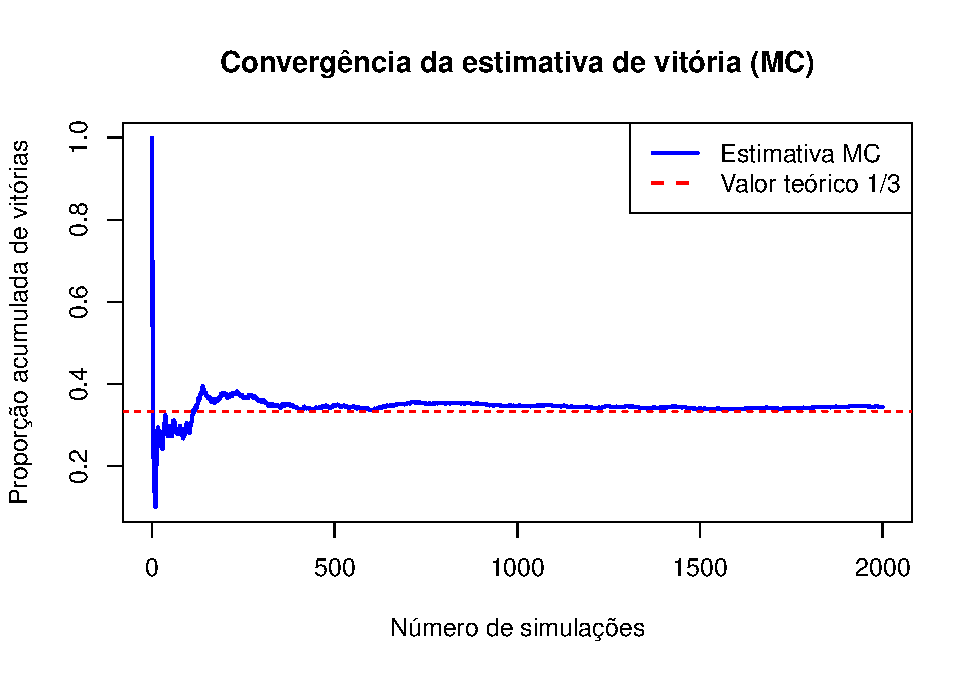
\includegraphics[keepaspectratio]{mc_files/figure-latex/unnamed-chunk-4-1.pdf}}}{}}\label{section}

\section{Quetão 8}\label{quetuxe3o-8}

\subsubsection{Suponha que tenhamos uma urna com bolas de mesmo tamanho
enumeradas de 1 à 100. Considere o experimento aleatório de retirar uma
bola da urna e observar o seu número até obtermos a bola com número
desejado. Nesse experimento, será considerado reposição, isto é, caso
não tenha sido observado a numeração desejada, a bola será devolvida à
urna. Implemente um procedimento de MC considerando 10 mil repetições
desse experimento e obtenha a média das retiradas necessárias para
obter-se o número desejado. Além disso, retorne uma aproximação da
probabilidade de se obter o número desejado. Dica: considere o número 77
como o número
desejado.}\label{suponha-que-tenhamos-uma-urna-com-bolas-de-mesmo-tamanho-enumeradas-de-1-uxe0-100.-considere-o-experimento-aleatuxf3rio-de-retirar-uma-bola-da-urna-e-observar-o-seu-nuxfamero-atuxe9-obtermos-a-bola-com-nuxfamero-desejado.-nesse-experimento-seruxe1-considerado-reposiuxe7uxe3o-isto-uxe9-caso-nuxe3o-tenha-sido-observado-a-numerauxe7uxe3o-desejada-a-bola-seruxe1-devolvida-uxe0-urna.-implemente-um-procedimento-de-mc-considerando-10-mil-repetiuxe7uxf5es-desse-experimento-e-obtenha-a-muxe9dia-das-retiradas-necessuxe1rias-para-obter-se-o-nuxfamero-desejado.-aluxe9m-disso-retorne-uma-aproximauxe7uxe3o-da-probabilidade-de-se-obter-o-nuxfamero-desejado.-dica-considere-o-nuxfamero-77-como-o-nuxfamero-desejado.}

\begin{Shaded}
\begin{Highlighting}[]
\FunctionTok{set.seed}\NormalTok{(}\DecValTok{123}\NormalTok{)}

\NormalTok{qtd\_simulacao }\OtherTok{\textless{}{-}} \DecValTok{10000}
\NormalTok{numero\_desejado }\OtherTok{\textless{}{-}} \DecValTok{77}
\NormalTok{qtd\_bolas\_totais }\OtherTok{\textless{}{-}} \DecValTok{100}

\NormalTok{retiradas }\OtherTok{\textless{}{-}} \FunctionTok{numeric}\NormalTok{(qtd\_simulacao)}

\ControlFlowTok{for}\NormalTok{ (i }\ControlFlowTok{in} \DecValTok{1}\SpecialCharTok{:}\NormalTok{qtd\_simulacao) \{}
\NormalTok{  vezes }\OtherTok{\textless{}{-}} \DecValTok{0}
\NormalTok{  bola\_retirada }\OtherTok{\textless{}{-}} \DecValTok{0}
  
  \ControlFlowTok{while}\NormalTok{ (bola\_retirada }\SpecialCharTok{!=}\NormalTok{ numero\_desejado) \{}
\NormalTok{    vezes }\OtherTok{\textless{}{-}}\NormalTok{ vezes }\SpecialCharTok{+} \DecValTok{1}
\NormalTok{    bola\_retirada }\OtherTok{\textless{}{-}} \FunctionTok{sample}\NormalTok{(}\DecValTok{1}\SpecialCharTok{:}\NormalTok{qtd\_bolas\_totais, }\DecValTok{1}\NormalTok{, }\AttributeTok{replace =} \ConstantTok{TRUE}\NormalTok{)}
\NormalTok{  \}}
  
\NormalTok{  retiradas[i] }\OtherTok{\textless{}{-}}\NormalTok{ vezes}
\NormalTok{\}}

\NormalTok{media\_retiradas }\OtherTok{\textless{}{-}} \FunctionTok{mean}\NormalTok{(retiradas)}
\NormalTok{probabilidade\_de\_desejada\_mc }\OtherTok{\textless{}{-}} \FunctionTok{mean}\NormalTok{(retiradas }\SpecialCharTok{==} \DecValTok{1}\NormalTok{)}

\FunctionTok{cat}\NormalTok{(}\StringTok{"Media das bolas retiradas: "}\NormalTok{, media\_retiradas, }\StringTok{"}\SpecialCharTok{\textbackslash{}n}\StringTok{"}\NormalTok{)}
\end{Highlighting}
\end{Shaded}

\begin{verbatim}
## Media das bolas retiradas:  101.0854
\end{verbatim}

\begin{Shaded}
\begin{Highlighting}[]
\FunctionTok{cat}\NormalTok{(}\StringTok{"Probabilidade do desejo: "}\NormalTok{, probabilidade\_de\_desejada\_mc, }\StringTok{"}\SpecialCharTok{\textbackslash{}n}\StringTok{"}\NormalTok{)}
\end{Highlighting}
\end{Shaded}

\begin{verbatim}
## Probabilidade do desejo:  0.0103
\end{verbatim}

\begin{center}\rule{0.5\linewidth}{0.5pt}\end{center}

\section{Questão 9}\label{questuxe3o-9}

\subsubsection{Um dono de cassino estuda disponibilizar um novo jogo e
solicita uma consultoria estatística para saber se o jogo será viável
para o cassino, isto é, se o valor esperado em dólares do lucro obtido
será positivo, em média. Realize uma simulação de MC considerando 100
mil jogos e obtenha o valor médio de lançamentos de um jogador bem como
a probabilidade (aproximada) de um jogador jogar apenas uma única
partida. Além disso, responda:Se um jogador paga \$10 dólares para jogar
e lucra \$1,50 dólares por cada jogada, o jogo é rentável para o dono do
cassino?}\label{um-dono-de-cassino-estuda-disponibilizar-um-novo-jogo-e-solicita-uma-consultoria-estatuxedstica-para-saber-se-o-jogo-seruxe1-viuxe1vel-para-o-cassino-isto-uxe9-se-o-valor-esperado-em-duxf3lares-do-lucro-obtido-seruxe1-positivo-em-muxe9dia.-realize-uma-simulauxe7uxe3o-de-mc-considerando-100-mil-jogos-e-obtenha-o-valor-muxe9dio-de-lanuxe7amentos-de-um-jogador-bem-como-a-probabilidade-aproximada-de-um-jogador-jogar-apenas-uma-uxfanica-partida.-aluxe9m-disso-respondase-um-jogador-paga-10-duxf3lares-para-jogar-e-lucra-150-duxf3lares-por-cada-jogada-o-jogo-uxe9-rentuxe1vel-para-o-dono-do-cassino}

\subsubsection{\texorpdfstring{\(\textbf{Regras do jogo: }\)}{\textbackslash textbf\{Regras do jogo: \}}}\label{textbfregras-do-jogo}

\begin{itemize}
\tightlist
\item
  Dois dados são lançados e caso a soma for 5, 6, 7, 8 ou 9 o jogo
  termina imediatamente;
\item
  Se nenhum dos resultamos acima for obtido, o jogador continua lançando
  ambos os dados até obter uma soma igual à 11 ou 12.
\end{itemize}

\begin{Shaded}
\begin{Highlighting}[]
\FunctionTok{set.seed}\NormalTok{(}\DecValTok{123}\NormalTok{) }

\NormalTok{qtd\_dados }\OtherTok{\textless{}{-}} \DecValTok{2}
\NormalTok{qtd\_simulacao }\OtherTok{\textless{}{-}} \DecValTok{100000} 
\NormalTok{vetor\_vencedor }\OtherTok{\textless{}{-}} \FunctionTok{c}\NormalTok{(}\DecValTok{5}\NormalTok{,}\DecValTok{6}\NormalTok{,}\DecValTok{7}\NormalTok{,}\DecValTok{8}\NormalTok{,}\DecValTok{9}\NormalTok{)}
\NormalTok{vetor\_perdeor }\OtherTok{\textless{}{-}} \FunctionTok{c}\NormalTok{(}\DecValTok{11}\NormalTok{,}\DecValTok{12}\NormalTok{)}

\NormalTok{qtd\_lancamentos }\OtherTok{\textless{}{-}} \FunctionTok{numeric}\NormalTok{(qtd\_simulacao)}
\NormalTok{terminou\_em\_uma\_jogada }\OtherTok{\textless{}{-}} \DecValTok{0}

\ControlFlowTok{for}\NormalTok{(i }\ControlFlowTok{in} \DecValTok{1}\SpecialCharTok{:}\NormalTok{qtd\_simulacao)\{}
\NormalTok{    vezes\_lancados }\OtherTok{\textless{}{-}} \DecValTok{1}
\NormalTok{    dados\_lancados\_soma }\OtherTok{\textless{}{-}} \FunctionTok{sum}\NormalTok{(}\FunctionTok{sample}\NormalTok{(}\DecValTok{1}\SpecialCharTok{:}\DecValTok{6}\NormalTok{, qtd\_dados, }\AttributeTok{replace =}\NormalTok{T))}

    \ControlFlowTok{if}\NormalTok{(dados\_lancados\_soma }\SpecialCharTok{\%in\%}\NormalTok{ vetor\_vencedor)\{}
\NormalTok{        terminou\_em\_uma\_jogada }\OtherTok{\textless{}{-}}\NormalTok{ terminou\_em\_uma\_jogada }\SpecialCharTok{+} \DecValTok{1}
\NormalTok{        qtd\_lancamentos[i] }\OtherTok{\textless{}{-}}\NormalTok{ vezes\_lancados}
        \ControlFlowTok{next}
\NormalTok{    \}}
    
    \ControlFlowTok{while}\NormalTok{(}\SpecialCharTok{!}\NormalTok{(dados\_lancados\_soma }\SpecialCharTok{\%in\%}\NormalTok{ vetor\_vencedor))\{}
\NormalTok{        dados\_lancados\_soma }\OtherTok{\textless{}{-}} \FunctionTok{sum}\NormalTok{(}\FunctionTok{sample}\NormalTok{(}\DecValTok{1}\SpecialCharTok{:}\DecValTok{6}\NormalTok{, qtd\_dados, }\AttributeTok{replace =}\NormalTok{T))}
\NormalTok{        vezes\_lancados }\OtherTok{\textless{}{-}}\NormalTok{ vezes\_lancados }\SpecialCharTok{+} \DecValTok{1}
\NormalTok{    \}}

\NormalTok{    qtd\_lancamentos[i] }\OtherTok{\textless{}{-}}\NormalTok{ vezes\_lancados}
\NormalTok{\}}

\NormalTok{media\_dos\_lancamentos }\OtherTok{\textless{}{-}} \FunctionTok{mean}\NormalTok{(qtd\_lancamentos)}
\NormalTok{probabilidade\_de\_uma\_jogada }\OtherTok{\textless{}{-}}\NormalTok{ terminou\_em\_uma\_jogada }\SpecialCharTok{/}\NormalTok{ qtd\_simulacao}

\FunctionTok{cat}\NormalTok{(}\StringTok{"média lançamento jogador:"}\NormalTok{, media\_dos\_lancamentos, }\StringTok{"}\SpecialCharTok{\textbackslash{}n}\StringTok{"}\NormalTok{)}
\end{Highlighting}
\end{Shaded}

\begin{verbatim}
## média lançamento jogador: 1.49581
\end{verbatim}

\begin{Shaded}
\begin{Highlighting}[]
\FunctionTok{cat}\NormalTok{(}\StringTok{"probabilidade de terminar em uma jogada:"}\NormalTok{, probabilidade\_de\_uma\_jogada, }\StringTok{"}\SpecialCharTok{\textbackslash{}n}\StringTok{"}\NormalTok{)}
\end{Highlighting}
\end{Shaded}

\begin{verbatim}
## probabilidade de terminar em uma jogada: 0.66702
\end{verbatim}

\begin{Shaded}
\begin{Highlighting}[]
\NormalTok{lucro\_cassino }\OtherTok{\textless{}{-}} \DecValTok{10} \SpecialCharTok{{-}}\NormalTok{ (}\FloatTok{1.5} \SpecialCharTok{*}\NormalTok{ qtd\_lancamentos)}
\NormalTok{lucro\_medio\_cassino }\OtherTok{\textless{}{-}} \FunctionTok{mean}\NormalTok{(lucro\_cassino)}

\FunctionTok{cat}\NormalTok{(}\StringTok{"lucro medio do cassino por jogador: $"}\NormalTok{, }\FunctionTok{round}\NormalTok{(lucro\_medio\_cassino, }\DecValTok{2}\NormalTok{), }\StringTok{"}\SpecialCharTok{\textbackslash{}n}\StringTok{"}\NormalTok{)}
\end{Highlighting}
\end{Shaded}

\begin{verbatim}
## lucro medio do cassino por jogador: $ 7.76
\end{verbatim}

\begin{Shaded}
\begin{Highlighting}[]
\ControlFlowTok{if}\NormalTok{(lucro\_medio\_cassino }\SpecialCharTok{\textgreater{}} \DecValTok{0}\NormalTok{)\{}
    \FunctionTok{cat}\NormalTok{(}\StringTok{"O jogo é rentável para o cassino.}\SpecialCharTok{\textbackslash{}n}\StringTok{"}\NormalTok{)}
\NormalTok{\} }\ControlFlowTok{else}\NormalTok{ \{}
    \FunctionTok{cat}\NormalTok{(}\StringTok{"O jogo NÃO é rentável para o cassino.}\SpecialCharTok{\textbackslash{}n}\StringTok{"}\NormalTok{)}
\NormalTok{\}}
\end{Highlighting}
\end{Shaded}

\begin{verbatim}
## O jogo é rentável para o cassino.
\end{verbatim}

\end{document}
